\part{Efeito dos aditivos hidrofílicos}
	
	Esta é a parte principal desta tese, onde a maior parte do tempo foi dedicada ao entendimento dos efeitos dos aditivos hidrofílicos no comportamento das micelas gigantes. Os resultados foram publicados na revista \emph{Journal of Colloid and Interface Science}, sob o título ``\emph{Rheological and calorimetric study of alkyltrimethylammonium bromide-sodium salicylate wormlike micelles in aqueous binary systems}".
	
	Serão apresentados inicialmente os resultados reológicos em função do efeito dos aditivos, e em seguida serão levantados alguns parâmetros que podem ser utilizados para descrever o efeito dos aditivos.
	
	Inicialmente, escolheu-se sacarose pois possui tipos de interação semelhantes à glicerina, e já havia sido testada em outros sistemas como, por exemplo, sistemas lamelares, onde teve o mesmo efeito da glicerina. 1,3-butanodiol (1,3BD) foi um aditivo escolhido devido a um estudo feito por Rami Abdel-Rahem, e seu estudo foi reproduzido e complementado com informações calorimétricas. Dimetilsulfóxido (DMSO) também é utilizado na literatura como um aditivo. A ureia é um aditivo que é frequentemente descrito na literatura como um agente desestruturante da água, que leva à desnaturação de proteínas.
	
	% todo: encontrar o motivo para DMSO.
	
	\chapter{Resultados}
		\section{Efeitos dos aditivos na reologia}
			
			A reologia é uma técnica que pode fornecer informações sobre a dinâmica de relaxação de um material, através da viscosidade. Em especial, o perfil de viscosidade em repouso (\(\eta_0\)) em função da concentração de cossoluto está relacionado com mudanças no processo de relaxação das micelas. Com o intuito de se estudar como a relaxação das micelas é afetado pelos aditivos, foram construídos vários diagramas de viscosidade em função da concentração de salicilato de sódio.
			
			Dos cinco aditivos selecionados, foram feitas comparações para realçar as diferenças e semelhanças entre os aditivos. Neste momento, os resultados serão discutidos com base somente no índice de refração das soluções. A figura \ref{fig:indice_refracao} mostra como o índice de refração das soluções com os aditivos variam em função da fração mássica de aditivo.
					
			\begin{figure}[h]
				\centering
				\includegraphics[width=0.7\textwidth]{imagens/propriedades/indice_refracao}
				\caption{Índice de refração em função da concentração de aditivo}
				\label{fig:indice_refracao}
			\end{figure}
	
			Inicialmente, comparou-se o sistema melhor estudado (glicerina) com sacarose, escolhida pois também possuía efeitos semelhantes à glicerina no intumescimento lamelar. A figura \ref{fig:rh_sacarose_glicerina} mostra os diagramas de viscosidade para soluções de micelas gigantes com 100 \mM{} de \CTAB, em concentrações crescentes de glicerina, e no ponto de igualdade no índice de refração de sacarose, 50\%.
			
			\begin{figure}[h]
				\centering
				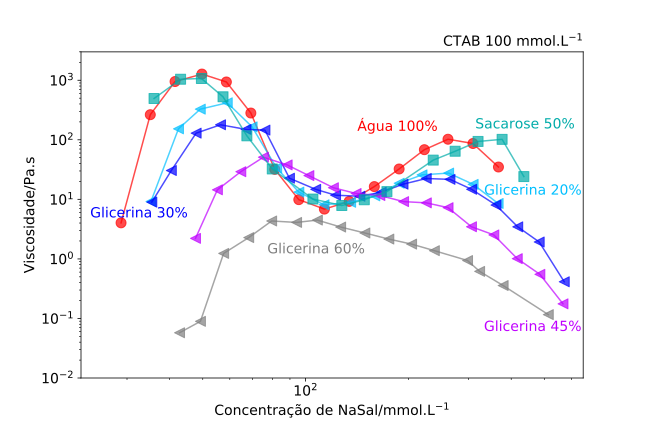
\includegraphics[width=0.7\textwidth]{imagens/reologia/RH_sacarose_glicerina}
				\caption{Viscosidade no repouso \(\eta_0\) em função da concentração de salicilato de sódio (NaSal) em várias concentrações dos aditivos glicerina e sacarose. 60\% de glicerina (V/V) e 50\% de sacarose (m/m) estão no ponto de equivalência do índice de refração.}
				\label{fig:rh_sacarose_glicerina}
			\end{figure} % todo: mencionar que curvas a laila mediu. Foram as de glicerina?
			
			Podemos observar que os dois picos de viscosidade observados em pequenas concentrações de glicerina, diminuem, e a região central permanece pouco afetada, como já havia sido descrito por Hoffmann. Porém, vemos que a adição de 50\% de sacarose praticamente não afetou a viscosidade das soluções, apesar da igualdade no índice de refração dessas soluções. Isso mostra que considerar somente o índice de refração não permite a previsão do comportamento dessas soluções, e isso motivou a realização de estudos posteriores.
			
			A figura \ref{fig:rh_13bd_dmso} mostra como os aditivos 1,3-butanodiol e dimetilsulfóxido afetam o perfil de viscosidade.
			
			\begin{figure}[h]
				\centering
				\includegraphics[width=0.7\textwidth]{imagens/reologia/RH_13BD_DMSO}
				\caption{Viscosidade no repouso \(\eta_0\) em função da concentração de salicilato de sódio (NaSal) em várias concentrações dos aditivos 1,3-butanodiol (1,3BD) e dimetilsulfóxido (DMSO). As concentrações de igualdade do índice de refração são 77\% (m/m) e 57\% (m/m), respectivamente}
				\label{fig:rh_13bd_dmso}
			\end{figure}
		
			O perfil de viscosidade dessas soluções foi muito mais afetado pelos aditivos do que era esperado observando-se somente o índice de refração, em especial o 1,3-butanodiol, onde 15\% (m/m) possui o mesmo efeito na viscosidade que 60\% de glicerina.
			
			A ureia possui o comportamento que mais difere dos outros aditivos, como mostra a figura \ref{fig:rh_ureia}.
			
			\begin{figure}[h]
				\centering
				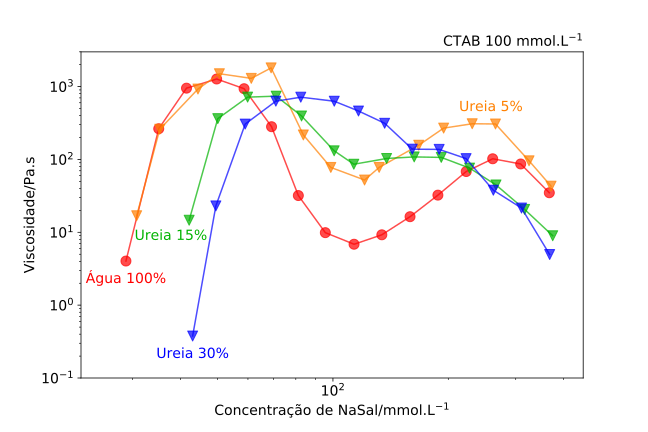
\includegraphics[width=0.7\textwidth]{imagens/reologia/RH_ureia}
				\caption{Viscosidade no repouso \(\eta_0\) em função da concentração de salicilato de sódio (NaSal) em várias concentrações de ureia. A concentração de igualdade de índice de refração é em torno de 55\%.}
				\label{fig:rh_ureia}
			\end{figure}

			Nesse caso, a viscosidade na região central aumentou, algo não observado nos outros cossolutos. Outro caso que possui um comportamento semelhante é o diagrama de orto-hidróxicinamato e \CTAB{} em pH 9. %todo: citar o artigo do OHCA
		
		\FloatBarrier
		
		\section{Efeito dos aditivos na calorimetria de micelas gigantes}
		
			A calorimetria de titulação isotérmica fornece informações sobre o quão favorável é a formação das micelas, através da concentração de formação de micelas gigantes, \cwlm. As figuras \ref{fig:itc_mg_glicerina} -- \ref{fig:itc_mg_ureia} mostram os perfis de formação de micelas gigantes para glicerina, sacarose, 1,3-butanodiol, dimetilsulfóxido e ureia.
		
			\begin{figure}[h]
				\centering
				\includegraphics[width=0.7\textwidth]{imagens/itc/ITC_MG_glic}
				\caption{Efeito da concentração de glicerina nas curvas de titulação de formação de micelas gigantes. A concentração de salicilato de sódio na cela de amostra é de 1,5\mM. A concentração do aditivo está em \% (V/V).}
				\label{fig:itc_mg_glicerina}
			\end{figure}  % todo: colocar a curva sem aditivo em todos. Trocar o 0% por uma curva preta.
			
			\begin{figure}[h]
				\centering
				\includegraphics[width=0.7\textwidth]{imagens/itc/ITC_MG_sac}
				\caption{Efeito da concentração de sacarose nas curvas de titulação de formação de micelas gigantes. A concentração de salicilato de sódio na cela de amostra é de 1,5\mM. A concentração do aditivo está em \% (m/m).}
				\label{fig:itc_mg_sacarose}
			\end{figure}
			
			As diferenças entre glicerina e sacarose, novamente, se evidenciaram. Da mesma maneira que na reologia, a presença de sacarose não afetou a formação de micelas gigantes. Já a glicerina teve um efeito deletério, aumentando significativamente a concentração necessária para o crescimento.
						
			\begin{figure}[h]
				\centering
				\includegraphics[width=0.7\textwidth]{imagens/itc/ITC_MG_13BD}
				\caption{Efeito da concentração de 1,3-butanodiol nas curvas de titulação de formação de micelas gigantes. A concentração de salicilato de sódio na cela de amostra é de 1,5\mM. A concentração do aditivo está em \% (m/m).}
				\label{fig:itc_mg_13bd}
			\end{figure}
			
			\begin{figure}[h]
				\centering
				\includegraphics[width=0.7\textwidth]{imagens/itc/ITC_MG_dmso}
				\caption{Efeito da concentração de dimetilsulfóxido nas curvas de titulação de formação de micelas gigantes. A concentração de salicilato de sódio na cela de amostra é de 1,5\mM. A concentração do aditivo está em \% (m/m).}
				\label{fig:itc_mg_dmso}
			\end{figure}  % todo: será que dá pra juntar os dois?

			1,3-BD e DMSO não se mostraram muito diferentes, apesar dos perfis reológicos serem bastante distintos, algo não totalmente inesperado, já que ambas as técnicas observam fenômenos diferentes. Isso indica que a queda de viscosidade com 1,3-BD não se deve à uma desestabilização micelar, o que levaria à uma diminuição na quantidade de micelas.

			\begin{figure}[h]
				\centering
				\includegraphics[width=0.7\textwidth]{imagens/itc/ITC_MG_ur}
				\caption{Efeito da concentração de ureia nas curvas de titulação de formação de micelas gigantes. A concentração de salicilato de sódio na cela de amostra é de 1,5\mM. A concentração do aditivo está em \% (m/m).}
				\label{fig:itc_mg_ureia}
			\end{figure}
		
			O comportamento da ureia seguiu o esperado, de acordo com a literatura, com um aumento de \cwlm{}. É interessante notar que o \DHwlm{} diminui com o aumento da concentração de ureia, o que sugere uma diminuição na adsorção de salicilato nas micelas. Em 35\% de ureia observa-se um perfil bastante diferente dos outros, porém nessa situação, ocorre a formação de um precipitado, cuja natureza será discutida na seção \ref{sec:cap_efeito_ureia}.
			
			Uma maneira de se resumir as curvas calorimétricas é através da concentração de formação de micelas gigantes (\cwlm) e a entalpia de micelização (\DHwlm). Dessa forma, podemos analisar o comportamento de todos os aditivos mais facilmente. A figura \ref{fig:cwlm_dhwlm_por_aditivo} resume isso, mostrando como essas propriedades variam com os aditivos, separadamente. A figura \ref{fig:cwlm_dhwlm_por_conc} mostra o mesmo, porém em função da concentração de aditivo.
			
			\begin{figure}[h]
				\begin{subfigure}[t]{0.5\textwidth}
					\centering
					\includegraphics[width=\textwidth]{imagens/itc/Cwlm_por_Aditivo}
					\caption{\cwlm{}}
					\label{fig:cwlm_por_aditivo}
				\end{subfigure}%
				\begin{subfigure}[t]{0.5\textwidth}
					\centering
					\includegraphics[width=\textwidth]{imagens/itc/DHwlm_por_Aditivo}
					\caption{\DHwlm{}}
					\label{fig:dhwlm_por_aditivo}
				\end{subfigure}
				\caption{\cwlm{} e \DHwlm{} em função dos aditivos e de sua concentração}
				\label{fig:cwlm_dhwlm_por_aditivo}
			\end{figure} 
		
			\begin{figure}[h]
				\begin{subfigure}[t]{0.5\textwidth}
					\centering
					\includegraphics[width=\textwidth]{imagens/itc/Cwlm_por_conc}
					\caption{\cwlm}
					\label{fig:cwlm_por_conc}
				\end{subfigure} %
				\begin{subfigure}[t]{0.5\textwidth}
					\centering
					\includegraphics[width=\textwidth]{imagens/itc/DHwlm_por_conc}
					\caption{\DHwlm}
					\label{fig:dhwlm_por_conc}
				\end{subfigure}
				
				\caption{\cmc{} e \DHmic{} em função da concentração de aditivo.}
				\label{fig:cwlm_dhwlm_por_conc}
			\end{figure}
		
		\FloatBarrier
		
		\section{Efeito dos aditivos na calorimetria de micelização}
		
		A calorimetria de formação de micelas gigantes possui uma complexidade maior devido à presença do salicilato. Para facilitar a interpretação, foram obtidas informações da formação de micelas esféricas, titulando-se \TTAB{} em água. As figuras \ref{fig:itc_glicerina} -- \ref{fig:itc_ureia} mostram as curvas de titulação para glicerina, sacarose, 1,3-butanodiol, dimetilsulfóxido e ureia.
					
%			\begin{figure}[h]
%				\centering
%				\includegraphics[width=0.7\textwidth]{imagens/itc/ITC_agua}
%				\caption{Titulação de \TTAB em água}
%				\label{fig:itc_agua}
%			\end{figure}
			
			\begin{figure}[h]
				\centering
				\includegraphics[width=0.7\textwidth]{imagens/itc/ITC_glic}
				\caption{Efeito da glicerina na titulação de \TTAB.}
				\label{fig:itc_glicerina}
			\end{figure}
		
			\begin{figure}[h]
				\centering
				\includegraphics[width=0.7\textwidth]{imagens/itc/ITC_sac}
				\caption{Efeito de sacarose na titulação de \TTAB}
				\label{fig:itc_sacarose}
			\end{figure}
			
			O efeito da glicerina na formação de micelas é semelhante ao efeito em micelas gigantes, exceto pelo aumento do \DHmic{}. Mais interessante, porém, é que sacarose levou à uma diminuição da \cmc{}. Isso levanta duas perguntas. Em primeiro lugar, qual é o mecanismo de estabilização micelar, e depois, porque esse mecanismo não afeta a formação de micelas gigantes?
			
			% todo: ref
			A literatura aponta que os grupos hidroxila pode interagir com a superfície micelar, diminuindo a repulsão entre as cabeças, estabilizando as micelas. Porém, nas micelas gigantes, o grupo carboxilato do salicilato se encontra nessa mesma região, então há uma competição entre esses dois grupos. Como o carboxilato é carregado, interage mais fortemente com as micelas e impede que a sacarose exerça sua influência estabilizadora. 
			
			\begin{figure}[h]
				\centering
				\includegraphics[width=0.7\textwidth]{imagens/itc/ITC_13BD}
				\caption{Efeito de 1,3-butanodiol na titulação de \TTAB}
				\label{fig:itc_13bd}
			\end{figure} 
		
			\begin{figure}[h]
				\centering
				\includegraphics[width=0.7\textwidth]{imagens/itc/ITC_dmso}
				\caption{Efeito de dimetilsulfóxido na titulação de \TTAB.}
				\label{fig:itc_dmso}
			\end{figure}
			
			Novamente, o 1,3-BD e DMSO mostraram possuir comportamentos semelhantes entre si, portanto o mecanismo que influencia ambas as micelas gigantes quanto esféricas deve ser semelhante.
			
			\begin{figure}[h]
				\centering
				\includegraphics[width=0.7\textwidth]{imagens/itc/ITC_ur}
				\caption{Efeito de ureia na titulação de \TTAB.}
				\label{fig:itc_ureia}
			\end{figure}
		
		A ureia influencia aumentando a \cmc{}, como esperado, porém não afeta muito o \DHmic{}. Logo, como não há \Sal{} para ser dessorvido das micelas, devido à alta constante dielétrica do meio, não há variações de \DHmic.
		
		As concentrações micelares críticas (\cmc) e entalpias de micelização (\DHmic) foram utilizadas para resumir as informações desta seção. A figura \ref{fig:cmc_dh_por_composto} mostra como as propriedades são afetadas pelos vários aditivos e suas concentrações, separadamente, e a figura \ref{fig:cmc_dh_por_conc} faz o mesmo, porém em função da concentração de aditivo.
		
		\begin{figure}[h]
			\begin{subfigure}[t]{0.5\textwidth}
				\centering
				\includegraphics[width=\textwidth]{imagens/itc/CMC_por_composto}
				\caption{\cmc}
				\label{fig:cmc_por_composto}
			\end{subfigure} %
			\begin{subfigure}[t]{0.5\textwidth}
				\centering
				\includegraphics[width=\textwidth]{imagens/itc/DH_por_composto}
				\caption{\DHmic}
				\label{fig:dh_por_composto}
			\end{subfigure}
		
			\caption{\cmc{} e \DHmic{} para os vários aditivos}
			\label{fig:cmc_dh_por_composto}
		\end{figure}

		\begin{figure}[h]
			\begin{subfigure}[t]{0.5\textwidth}
				\centering
				\includegraphics[width=\textwidth]{imagens/itc/ITC_cmc_adit}
				\caption{\cmc}
				\label{fig:cmc_por_conc}
			\end{subfigure} %
			\begin{subfigure}[t]{0.5\textwidth}
				\centering
				\includegraphics[width=\textwidth]{imagens/itc/ITC_DH_adit}
				\caption{\DHmic}
				\label{fig:dh_por_conc}
			\end{subfigure}
			
			\caption{\cmc{} e \DHmic{} em função da concentração de aditivo.}
			\label{fig:cmc_dh_por_conc}
		\end{figure}
	
		\FloatBarrier
		
	\chapter{Parâmetros a serem estudados}
		\section{Índice de refração}

		A figura \ref{fig:indice_refracao} mostrou como o índice de refração varia com a concentração de aditivo. Como os resultados reológicos evidenciaram, considerar somente o índice de refração não é uma maneira muito boa para explicar o comportamento reológico.
		
		Caso contrário, haveria um padrão notável num gráfico comparativo das concentrações e entalpias. Isso está evidenciado nas figuras \ref{fig:cmc_dh_por_n} e \ref{fig:cwlm_dhwlm_por_n}, onde não há um padrão geral observado para todos os aditivos.
		
		\begin{figure}[h]
			\begin{subfigure}[t]{0.5\textwidth}
				\centering
				\includegraphics[width=\textwidth]{imagens/itc/Cwlm_por_n}
				\caption{\cwlm}
				\label{fig:cwlm_por_n}
			\end{subfigure} %
			\begin{subfigure}[t]{0.5\textwidth}
				\centering
				\includegraphics[width=\textwidth]{imagens/itc/DHwlm_por_n}
				\caption{\DHwlm}
				\label{fig:dhwlm_por_n}
			\end{subfigure}
			
			\caption{\cwlm{} e \DHwlm{} em função do índice de refração.}
			\label{fig:cwlm_dhwlm_por_n}
		\end{figure}
		
		\begin{figure}[h]
			\begin{subfigure}[t]{0.5\textwidth}
				\centering
				\includegraphics[width=\textwidth]{imagens/itc/CMC_por_n}
				\caption{\cmc}
				\label{fig:cmc_por_n}
			\end{subfigure} %
			\begin{subfigure}[t]{0.5\textwidth}
				\centering
				\includegraphics[width=\textwidth]{imagens/itc/DH_por_n}
				\caption{\DHmic}
				\label{fig:dh_por_n}
			\end{subfigure}
			
			\caption{\cmc{} e \DHmic{} em função do índice de refração.}
			\label{fig:cmc_dh_por_n}
		\end{figure}

		Comparando-se as figuras \ref{fig:cwlm_dhwlm_por_n} e \ref{fig:cmc_dh_por_n}, pode-se observar que há uma correlação entre a formação de micelas gigantes e as concentrações críticas. Aparentemente há um grupo composto de 1,3BD, DMSO e ureia. Glicerina e sacarose se comportam bastante diferentemente, sendo que sacarose possui o comportamento mais diferenciado, não havendo mudança na \cwlm{} e uma diminuição da \cmc{}.
		
		Agrupamentos desse tipo não podem ser feitos com as entalpias, que parecem ter valores bastante variáveis. Porém, é necessário enfatizar que os valores de entalpia obtidos para a formação de micelas gigantes não são tão confiáveis quanto os de formação de micelas esféricas, já que estendeu-se a faixa de concentração de titulante, de modo a obter o perfil calorimétrico completo de todas as amostras. Isso reduz a precisão nos valores de entalpia iniciais. Esse problema possui menor relevância para \cwlm{}, que foi definida como sendo o ponto mínimo da curva, não uma subtração de duas regiões pré e pós-micelar. Apesar disso, o padrão observado para as mudanças de entalpia na presença de ureia podem ser explicadas pelo aumento da constante dielétrica do meio, como previamente mencionado.

		\FloatBarrier
		
		\section{Constante dielétrica}
		
		A constante dielétrica está relacionada ao grau de dissociação de espécies iônicas em solução. Quanto maior a constante, maior o grau de dissociação. Isso resulta, por exemplo, no aumento da \cmc{} pois há menos contraíons para reduzir a carga superficial micelar. A contribuição desse parâmetro já havia sido levantada em um estudo anterior. % todo: ref.
		A figura \ref{fig:cte_dieletrica} mostra como a constante dielétrica varia em função da concentração de aditivo. 
		
		\begin{figure}[h]
			\centering
			\includegraphics[width=0.7\textwidth]{imagens/propriedades/cte_dieletrica}
			\caption{Constante dielétrica em função da concentração de aditivo}
			\label{fig:cte_dieletrica}
		\end{figure}
	
		Da mesma maneira que o índice de refração, as concentrações micelares e entalpias dos processos serão comparados com a constante dielétrica do meio para tentar observar algum padrão.
		
		\begin{figure}[h]
			\begin{subfigure}[t]{0.5\textwidth}
				\centering
				\includegraphics[width=\textwidth]{imagens/itc/Cwlm_por_eps}
				\caption{\cwlm}
				\label{fig:cwlm_por_eps}
			\end{subfigure} %
			\begin{subfigure}[t]{0.5\textwidth}
				\centering
				\includegraphics[width=\textwidth]{imagens/itc/DHwlm_por_eps}
				\caption{\DHwlm}
				\label{fig:dhwlm_por_eps}
			\end{subfigure}
			
			\caption{\cwlm{} e \DHwlm{} em função da constante dielétrica \(\varepsilon\).}
			\label{fig:cwlm_dhwlm_por_eps}
		\end{figure}
		
		\begin{figure}[h]
			\begin{subfigure}[t]{0.5\textwidth}
				\centering
				\includegraphics[width=\textwidth]{imagens/itc/CMC_por_eps}
				\caption{\cmc}
				\label{fig:cmc_por_eps}
			\end{subfigure} %
			\begin{subfigure}[t]{0.5\textwidth}
				\centering
				\includegraphics[width=\textwidth]{imagens/itc/DH_por_eps}
				\caption{\DHmic}
				\label{fig:dh_por_eps}
			\end{subfigure}
			
			\caption{\cmc{} e \DHmic{} em função da constante dielétrica \(\varepsilon\).}
			\label{fig:cmc_dh_por_eps}
		\end{figure}
		
		\FloatBarrier
		\section{Parâmetro de Gordon}
		\section{Interação dos aditivos com a superfície micelar}
		\section{Decomposição em propriedades fundamentais}
	\chapter{Correlações entre os parâmetros e as propriedades}
		\section{Reologia}
		\section{Calorimetria}
